%===============================================================================
% Template Name:      CDE Thesis Presentation template
% Template URI:       http://github.com/csaybar/cde-thesis/
% Description:        Starter Presentation template for CDE master thesis 
% Version:            1.1.1
% Author:             Johan Janse van Rensburg
% Modified by:        Cesar Aybar
% License:            MIT License
% License URI:        http://opensource.org/licenses/MIT
%===============================================================================


%=================================================
% theme and color
%=================================================
\documentclass[compress]{beamer}
\usepackage{amsfonts,amsmath,oldgerm}
\usetheme{sintef}
\usepackage{graphicx}
\usepackage{animate}
\usepackage[labelformat=empty]{caption}
 	
\usetheme{Warsaw} % Themes http://www.hartwork.org/beamer-theme-matrix/
\usefonttheme[onlymath]{serif}



%=================================================
% packages and new commands
%=================================================
\usepackage[ruled, linesnumbered, vlined]{algorithm2e}
\usepackage{epsfig, subfigure, amssymb, multirow, algorithmic, amsmath}
\newcommand*{\superscript}[1]{\ensuremath{^{\rm #1}}}
\newcommand*{\subscript}[1]{\ensuremath{_{\rm #1}}}

%=================================================
% thesis details (first slide)
%=================================================
\title[{\sc How reliable are SEN2 cloud detection algorithms?} \hspace{0.8cm} \insertframenumber/\inserttotalframenumber]{{\sc How reliable are SEN2 cloud detection algorithms?}}
\subtitle{Global uncertainty estimation using Deep Kernel Learning.}
\author{\href{mailto:csaybar@gmail.com}{Cesar Luis Aybar Camacho}}
\institute{\textbf{Erasmus Mundus Joint Master Degree Programme \\ Copernicus Master in Digital Earth} \\ Specialization track GeoData Science}
\date{Vannes, France, 2022}


%=================================================
% start presentation
%=================================================
\begin{document}
	
%========================
% title page
%========================
\begingroup
\setbeamertemplate{headline}{}
\addtobeamertemplate{frametitle}{\vskip-1.7ex}{}
\begin{frame}
	\begin{center}
		\vspace{0.1cm}
		
\includegraphics[scale=0.15]{images/logo.pdf}
	\end{center}
	\titlepage
\end{frame}
\endgroup

%========================
% your slides:
%========================
\begin{frame}
	\frametitle{Acknowledge}
	\begin{center}
		\vspace{0.1cm}
		
\includegraphics[scale=0.25]{images/acknowledge.pdf}
	\end{center}
\end{frame}

\section{Problem definition}
\begin{frame}{Problem definition}
	\begin{center}
		\begin{figure}
			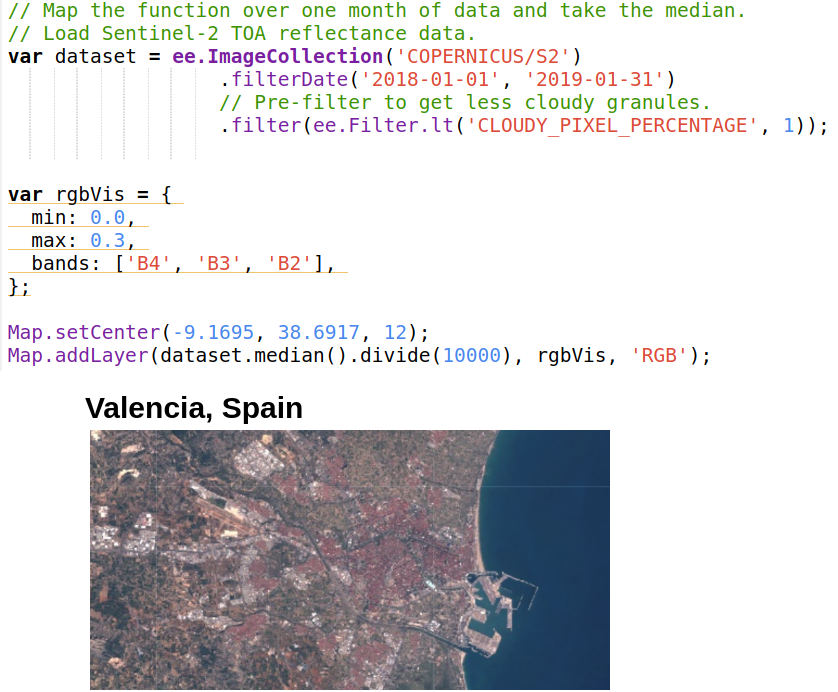
\includegraphics[width=0.76\linewidth]{images/problematic_01.png}
		\end{figure}
	\end{center}
\end{frame}


\begin{frame}{Problem definition}
	\begin{center}
		\begin{figure}
			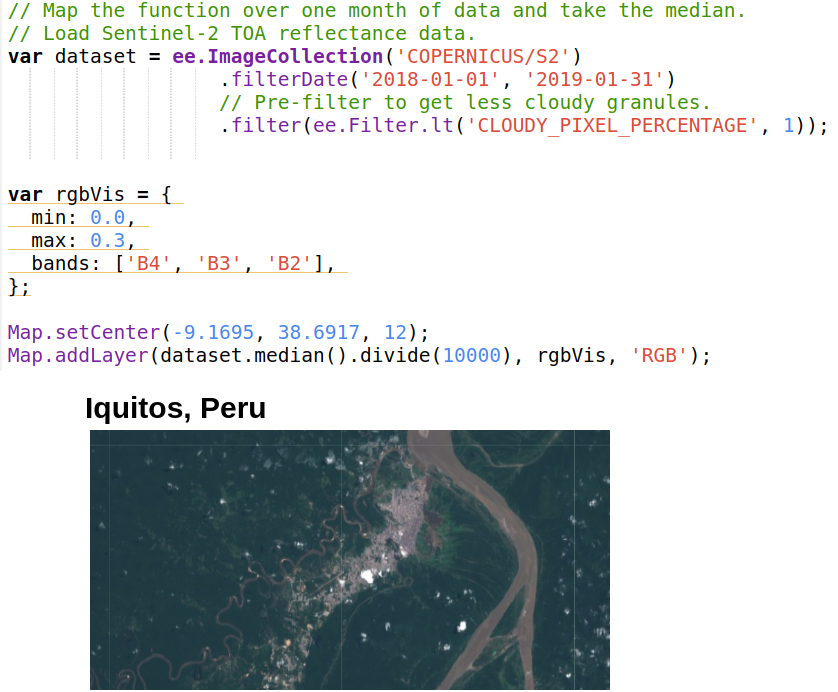
\includegraphics[width=0.76\linewidth]{images/problematic_02.png}
		\end{figure}
	\end{center}
\end{frame}


\begin{frame}{Problem definition}
	\begin{center}
		\begin{figure}
			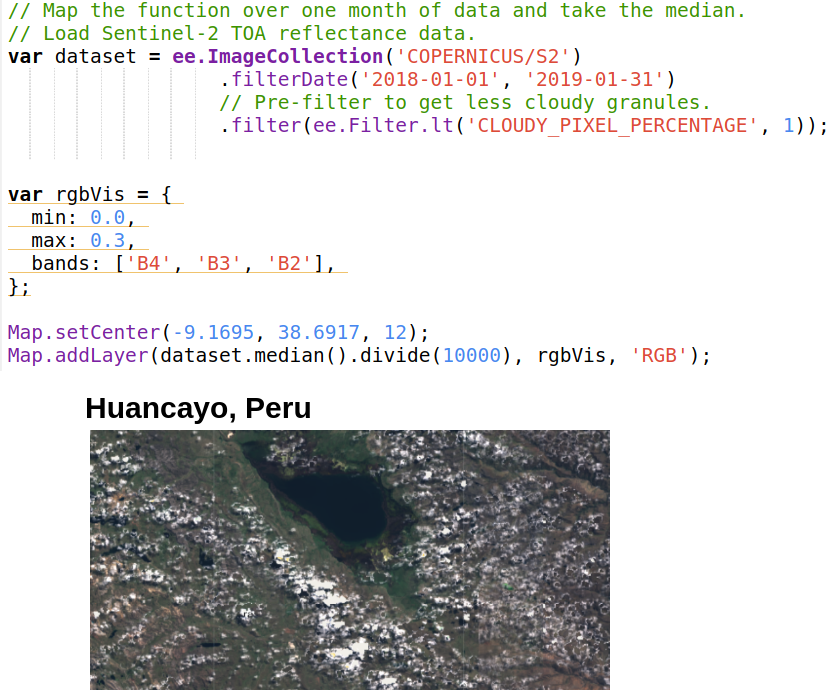
\includegraphics[width=0.76\linewidth]{images/problematic_03.png}
		\end{figure}
	\end{center}
\end{frame}


\begin{frame}{Problem definition}
	\begin{center}
		\textbf{\Large{Is it possible to predict cloud cover more accurately?}}\\
	\end{center}
\end{frame}

\begin{frame}{Problem definition}
	\begin{center}
		\textcolor{gray}{\large{Is it possible to predict cloud cover more accurately?}}\\
		\textcolor{red}{\textbf{\Large{How do cloud cover algorithms work?}}}
		
	\end{center}
\end{frame}


\begin{frame}{Problem definition}
	\begin{center}
		\textcolor{gray}{\large{Is it possible to predict cloud cover more accurately?}}\\
		\textcolor{gray}{\large{How do cloud cover algorithms work?}}\\
		\textcolor{red}{\textbf{\Large{What is a cloud?}}}				
	\end{center}
\end{frame}


\section{Intro}
\begin{frame}{What is a cloud?}
	\begin{center}
		\begin{figure}
			\centering
			
\includegraphics[width=0.8\linewidth]{images/intro_fig00_0.png}
			\label{fig:introfig01}
	\end{figure}
	\vspace{20px}
	\textbf{A cloud is a mass of water drops or ice crystals suspended in the atmosphere.}	
	\end{center}
\end{frame}


\begin{frame}{What is a cloud?}
	\begin{center}
		\begin{figure}
			\centering
			\includegraphics[width=0.7\linewidth]{images/cloud_types.pdf}
			\label{fig:introfig01}
		\end{figure}
		\textbf{A cloud is a mass of water drops or ice crystals suspended in the atmosphere.}	
	\end{center}
\end{frame}


\begin{frame}{What is a cloud?}
	\begin{center}
		\begin{figure}
			\centering
			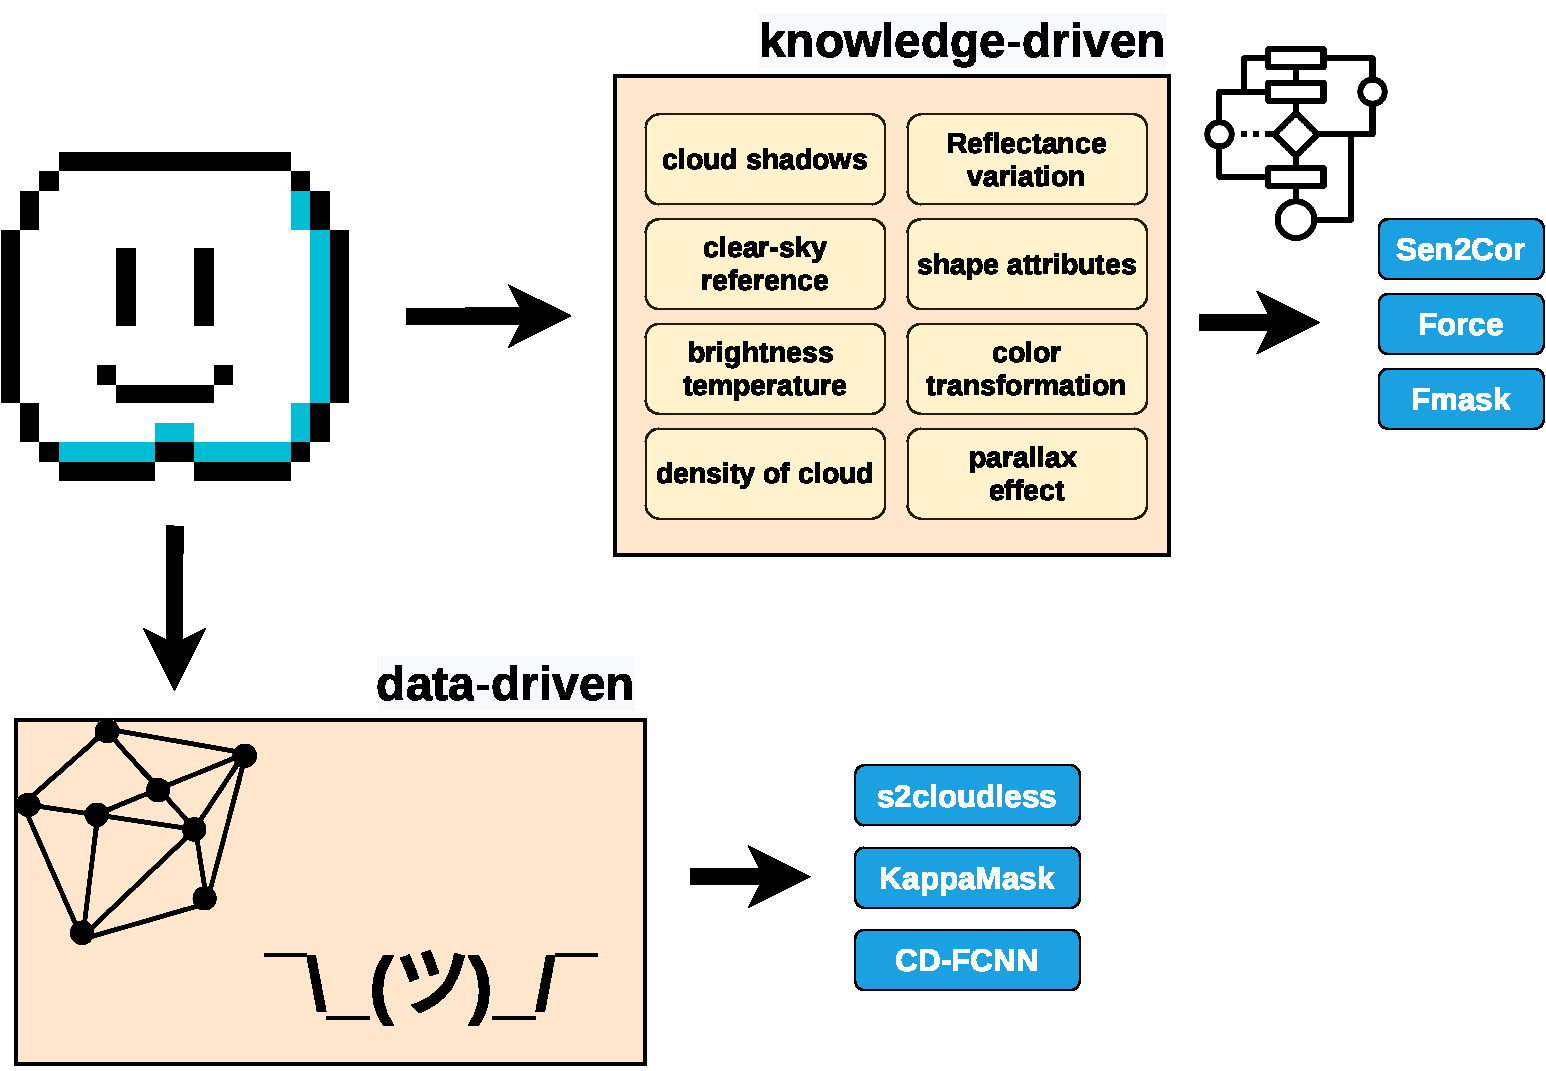
\includegraphics[width=0.85\linewidth]{images/intro_what_is_a_cloud.pdf}
			\label{fig:introfig01}
		\end{figure}
	\end{center}
\end{frame}


\begin{frame}{Context - I}
	\begin{center}
		\begin{figure}
			\centering
			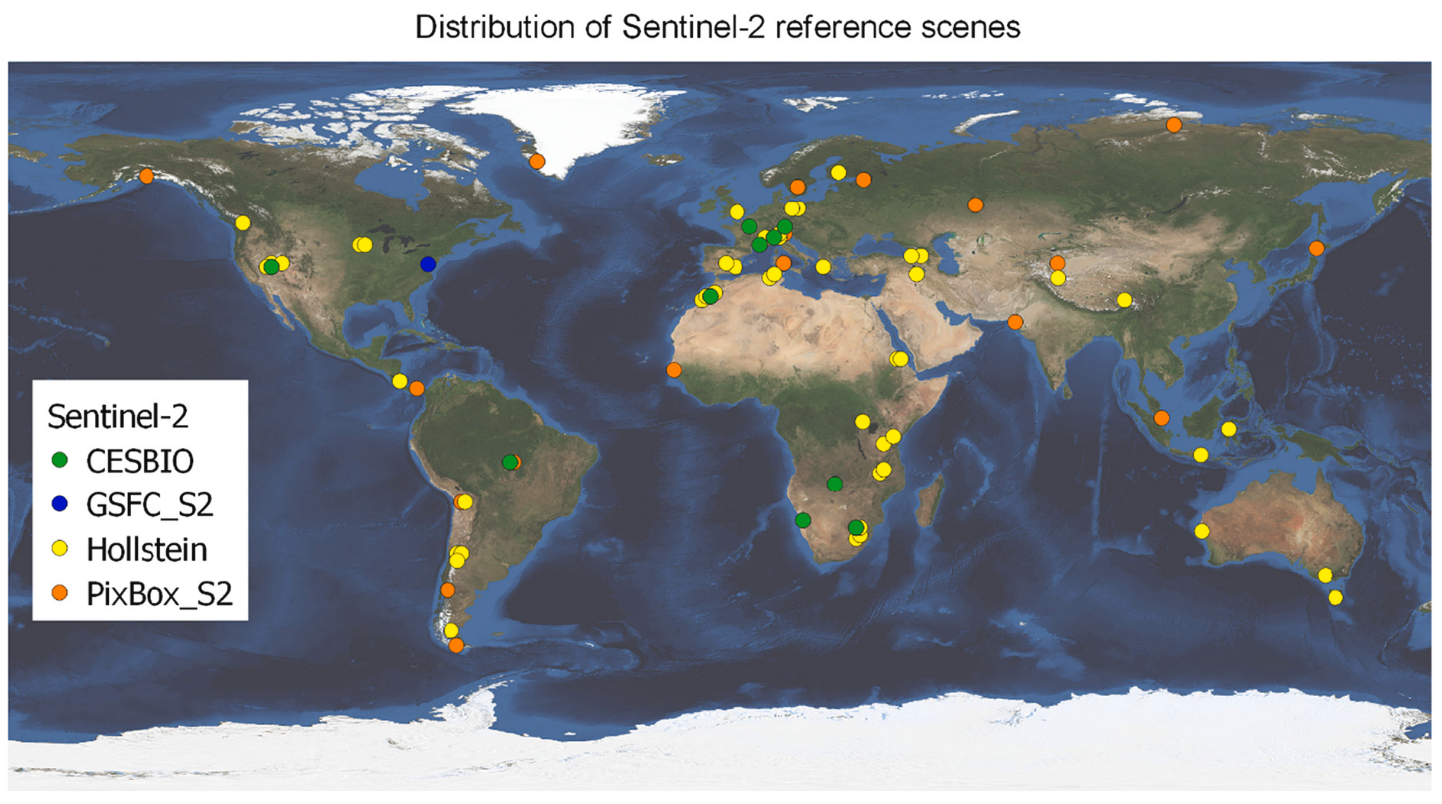
\includegraphics[width=0.85\linewidth]{images/intro_fig01.png}
			\caption[fig:introfig01]{Geographical distribution reference cloud detection datasets for Sentinel-2 (Skakun et al. 2022).}
			\label{fig:introfig01}
		\end{figure}
	\end{center}
\end{frame}


\begin{frame}{Context - II}
	\begin{columns}
		\begin{column}{0.5\textwidth}
			\begin{figure}
				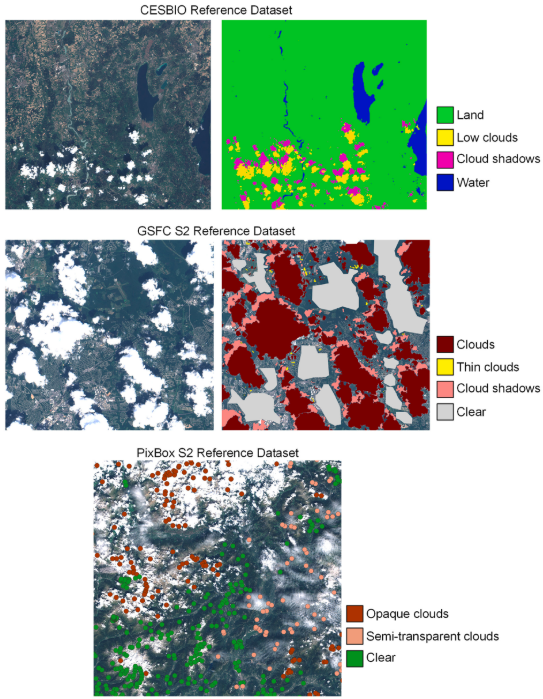
\includegraphics[width=0.85\textwidth]{images/contex_I.png}
				\caption[fig:introfig01]{Skakun et al. 2022}				
				\label{fig:introfig02}
			\end{figure}	
		\end{column}
		\begin{column}{0.5\textwidth}
			\begin{itemize}
				\item Cloud labels created by human photo-interpretation and ground-based camaras.
			\end{itemize}
		\end{column}
	\end{columns}
\end{frame}


\begin{frame}{Context - II}
	\begin{columns}
		\begin{column}{0.5\textwidth}
			\begin{figure}
				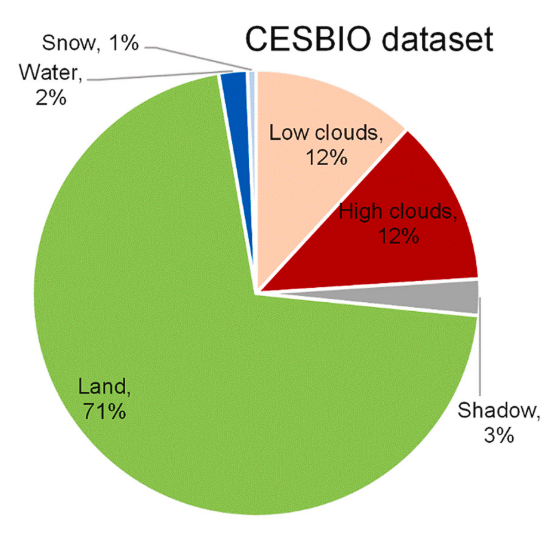
\includegraphics[width=0.85\textwidth]{images/contex_II.png}
				\caption[fig:introfig01]{Skakun et al. 2022}				
				\label{fig:introfig02}
			\end{figure}	
		\end{column}
		\begin{column}{0.5\textwidth}
			\begin{itemize}
				\item Cloud labels created by human photo-interpretation and ground-based camaras.
				\item High class imbalance.
			\end{itemize}
		\end{column}
	\end{columns}
\end{frame}

\begin{frame}{Context - II}
	\begin{columns}
		\begin{column}{0.5\textwidth}
			\begin{figure}
				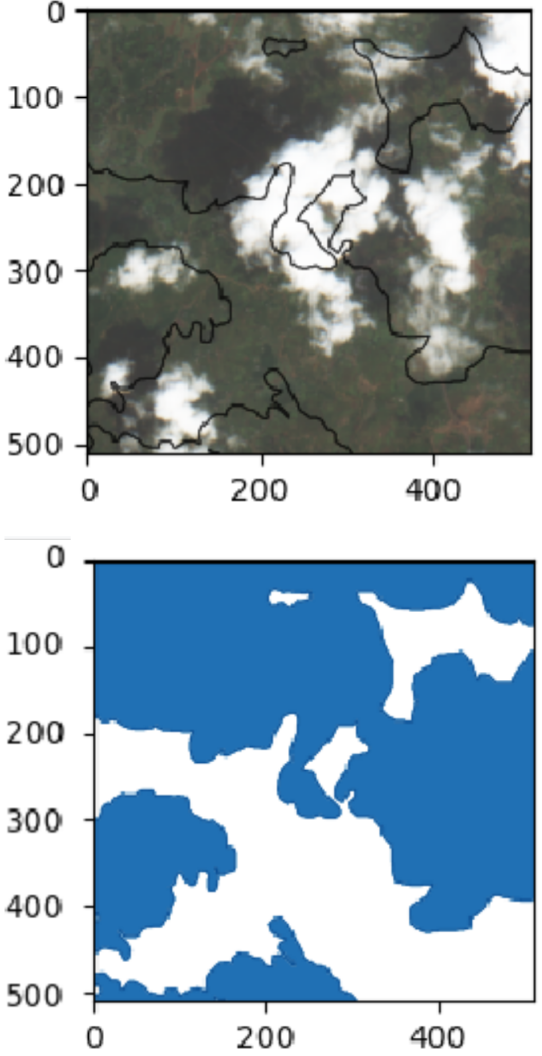
\includegraphics[width=0.6\textwidth]{images/contex_III.png}
				\caption[fig:introfig01]{Skakun et al. 2022}				
				\label{fig:introfig02}
			\end{figure}	
		\end{column}
		\begin{column}{0.5\textwidth}
			\begin{itemize}
				\item Cloud labels created by human photo-interpretation, active learning and ground-based camaras.
				\item High class imbalance.
				\item \textbf{The quality of some datasets is poor.}
			\end{itemize}
		\end{column}
	\end{columns}
\end{frame}




\begin{frame}{Context - II}
	\begin{columns}
		\begin{column}{0.5\textwidth}
			\begin{figure}
				\includegraphics[width=0.95\textwidth]{images/intro_fig02_2.png}
				\label{fig:introfig02}
			\end{figure}	
		\end{column}
		\begin{column}{0.5\textwidth}
			\begin{itemize}
				\item Cloud labels created by human photo-interpretation and ground-based camaras.
				\item High class imbalance.	
				\item \textbf{The quality of some datasets is poor.}
				\item Created by \textbf{\textit{closed science practices}}.
				\item \textbf{No temporal features}.
			\end{itemize}
		\end{column}
	\end{columns}
\end{frame}



\section{Data}
\begin{frame}
	\begin{center}
		\begin{figure}
			\animategraphics[width=0.55\linewidth,loop,autoplay]{10}{images/gif01/frame-}{0}{6}
		\end{figure}
		\textcolor{blue}{\href{https://cloudsen12.github.io/}{https://cloudsen12.github.io/}}
	\end{center}
\end{frame}


\begin{frame}{CloudSEN12 - Team <3}
	\begin{center}
		\begin{figure}
			\centering
			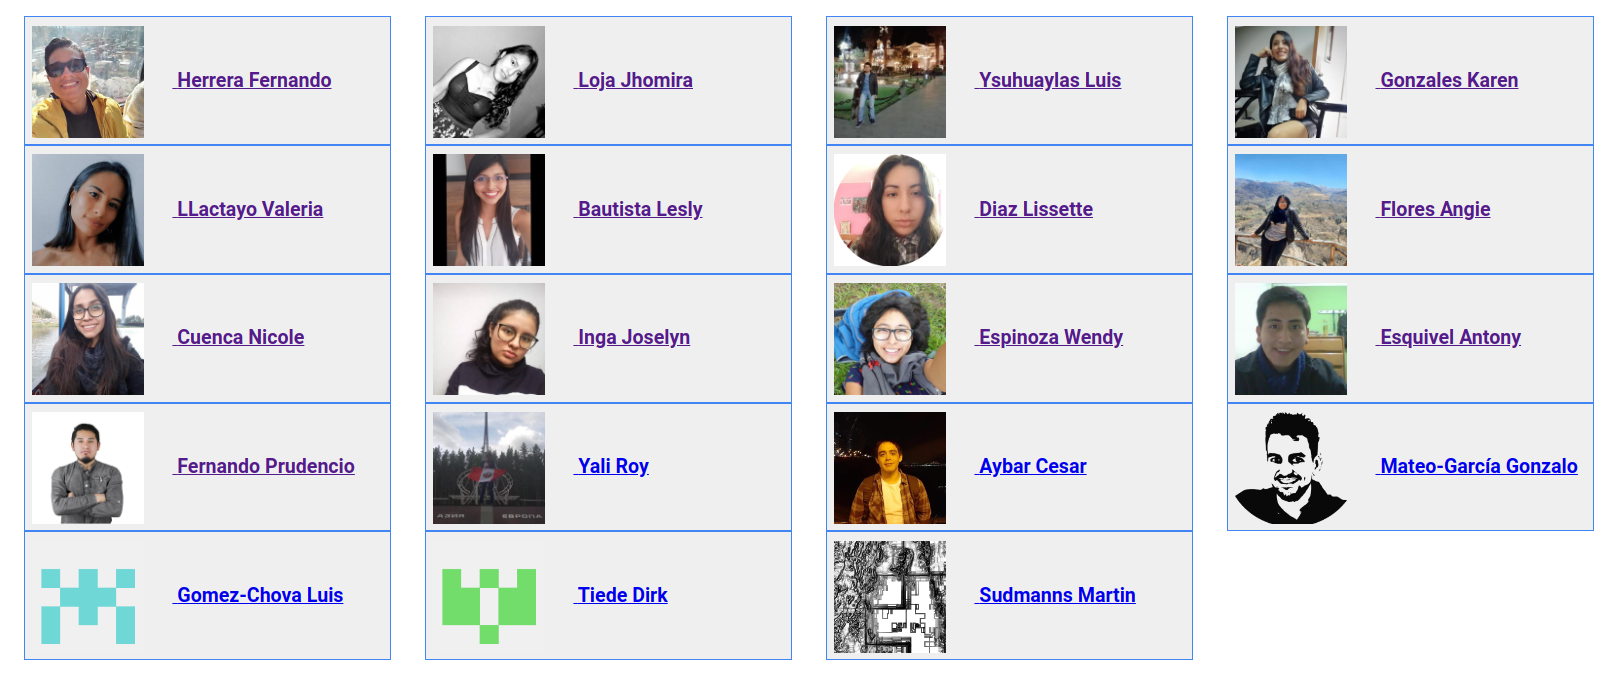
\includegraphics[width=1.0\linewidth]{images/dataset_team.png}
			{\caption*{CloudSEN12 team}}
			\label{fig:introfig01}
		\end{figure}
	\end{center}
\end{frame}


\begin{frame}{CloudSEN12 - Map}
	\begin{center}
		\begin{figure}
			\centering
			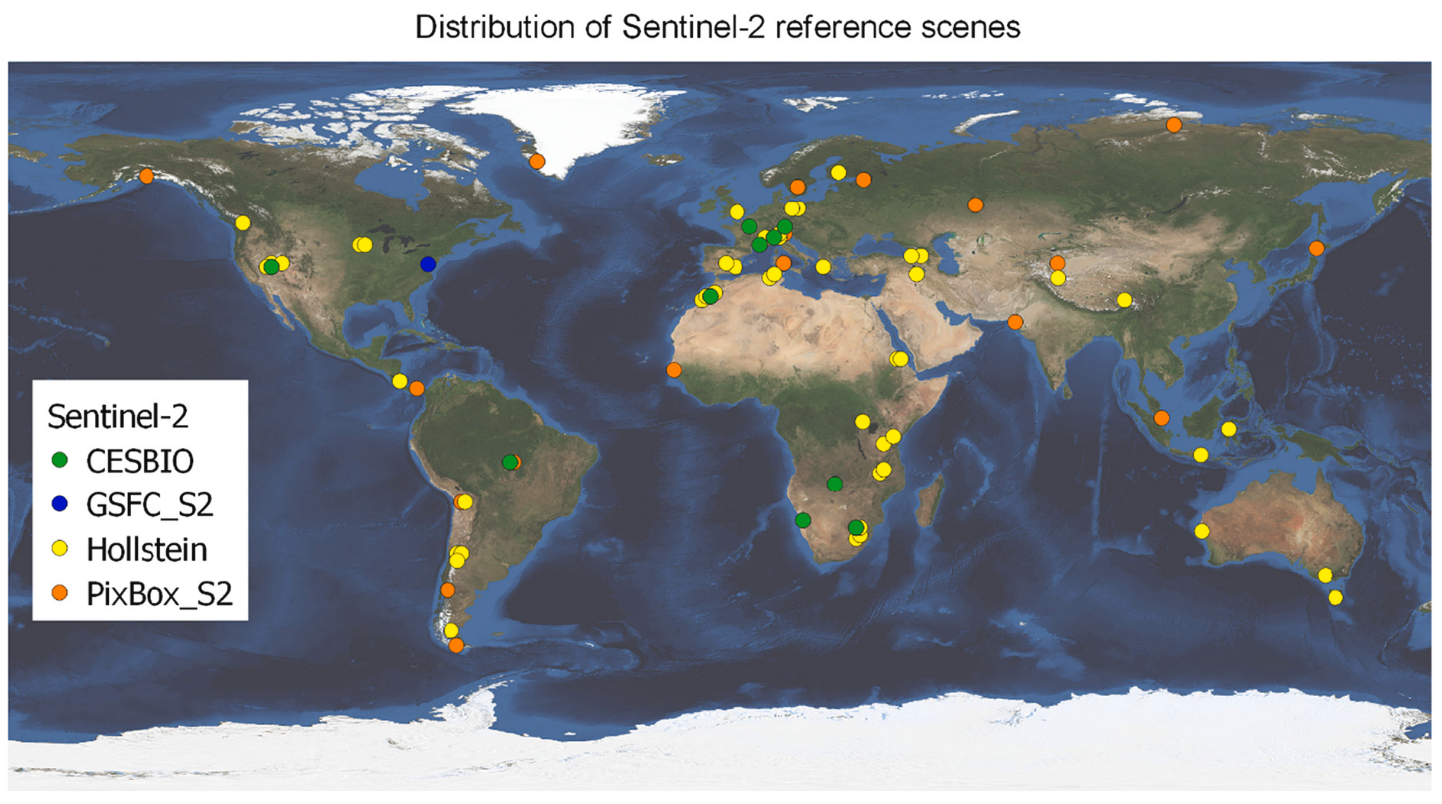
\includegraphics[width=0.85\linewidth]{images/intro_fig01.png}
			\caption[fig:introfig01]{Geographical distribution reference cloud detection datasets for Sentinel-2 (Skakun et al. 2022).}
			\label{fig:introfig01}
		\end{figure}
	\end{center}
\end{frame}

\begin{frame}{CloudSEN12 - Map}
	\begin{center}
		\begin{figure}
			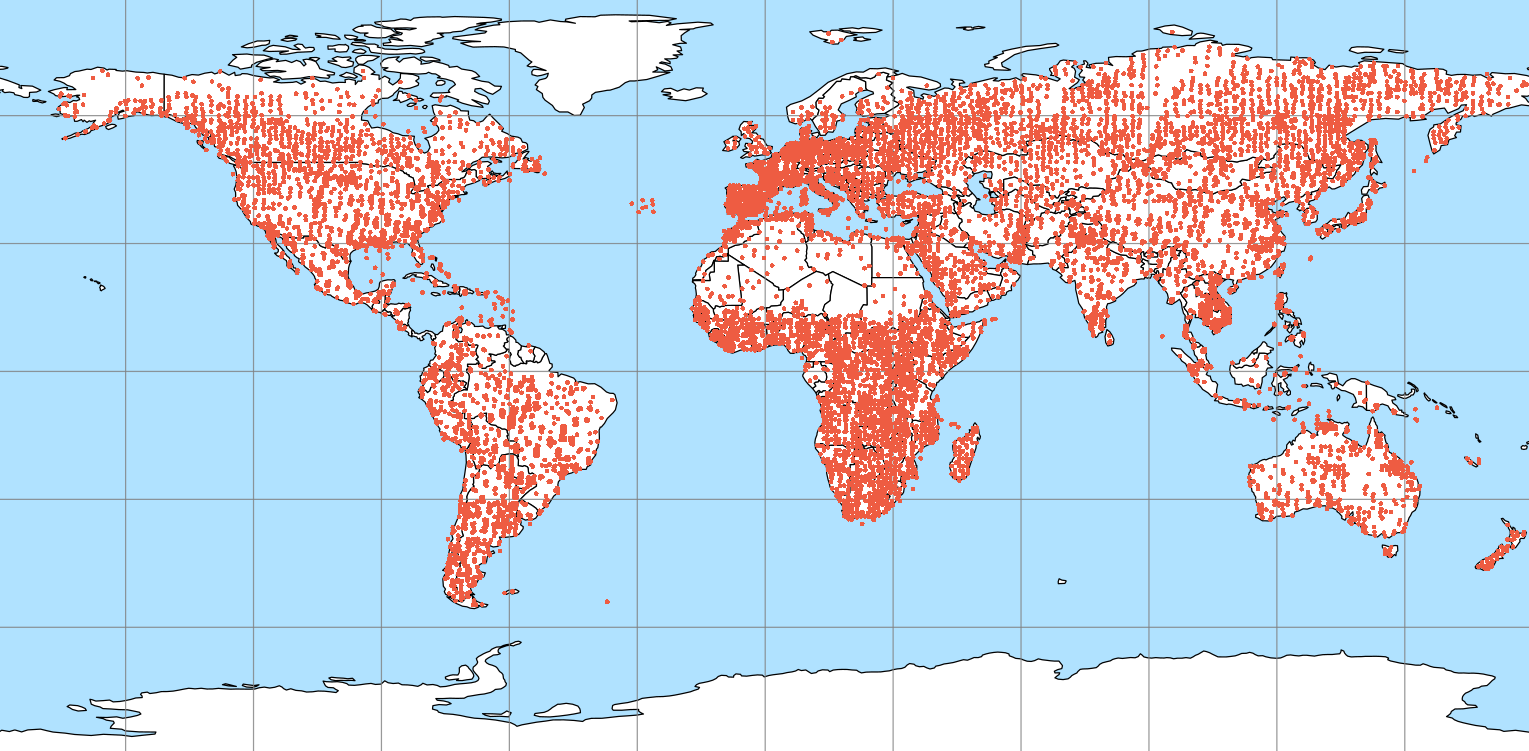
\includegraphics[width=0.85\linewidth]{images/intro_fig04.png}
			\caption[fig:introfig04]{CloudSEN12 spatial distribution}
		\end{figure}
	\end{center}
\end{frame}


\begin{frame}{CloudSEN12 - Data preparation}
	\begin{columns}
		\begin{column}{0.6\textwidth}
			\begin{figure}
				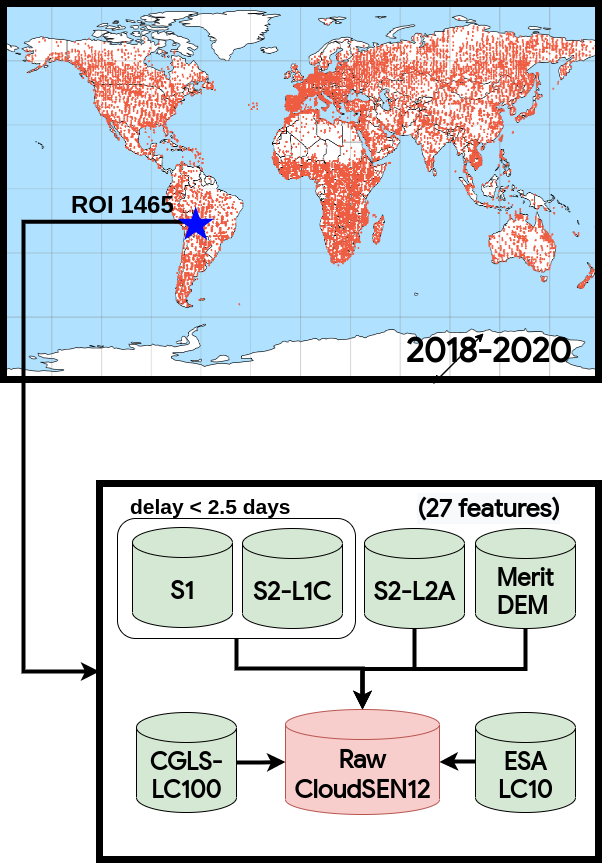
\includegraphics[width=0.6\textwidth]{images/methodology01.png}
				\label{fig:introfig02}
			\end{figure}
		\end{column}
		\begin{column}{0.4\textwidth}
			\begin{itemize}
				\item Merging of different spatio-temporal datasets to use as predictors.
				\item Semi-automatic selection of ROIs (5090x5090 m.)
			\end{itemize}
		\end{column}
	\end{columns}
\end{frame}




\begin{frame}{CloudSEN12 - Data Selection}
	\begin{columns}
		\begin{column}{0.7\textwidth}
			\begin{figure}
				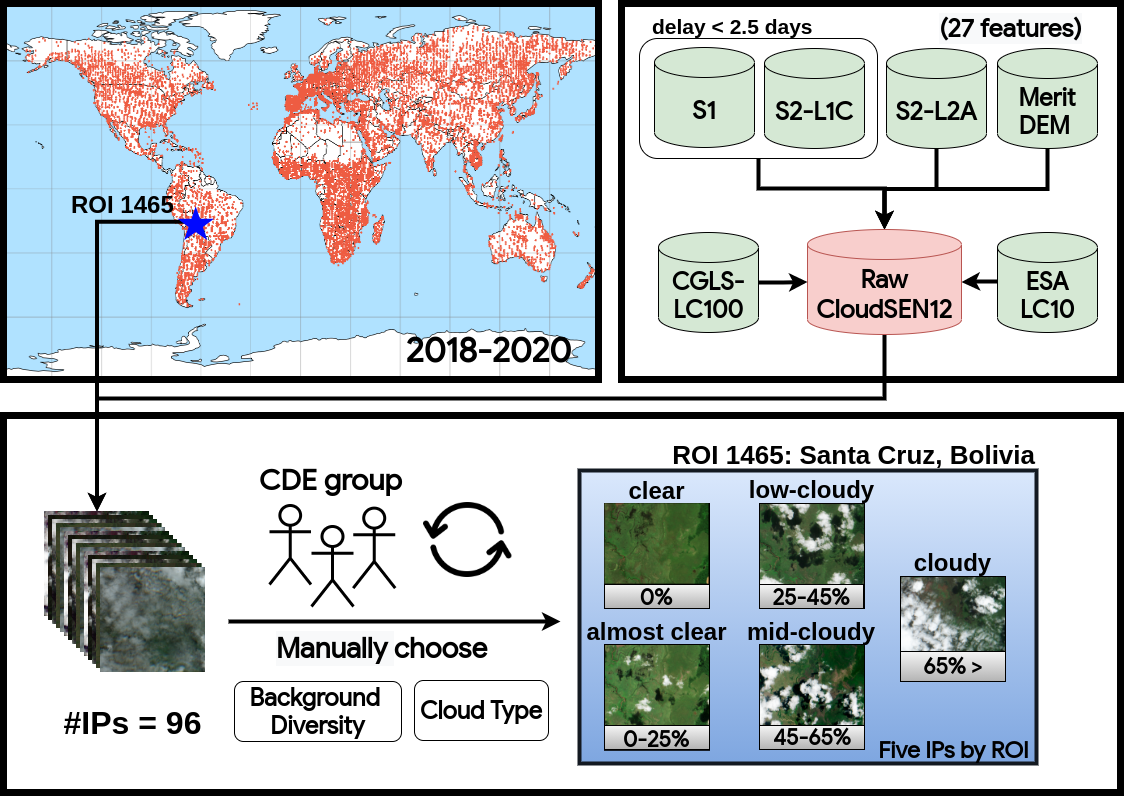
\includegraphics[width=1\textwidth]{images/methodology02.png}
				\label{fig:introfig02}
			\end{figure}
		\end{column}
		\begin{column}{0.3\textwidth}
			\begin{itemize}
				\item Each ROI have multiple IPs. We manually select five IPs considering the background, cloud type, and cloud coverage.
			\end{itemize}
		\end{column}
	\end{columns}
\end{frame}


\begin{frame}{CloudSEN12 - Labeling}
	\begin{columns}
		\begin{column}{0.7\textwidth}
			\begin{figure}
				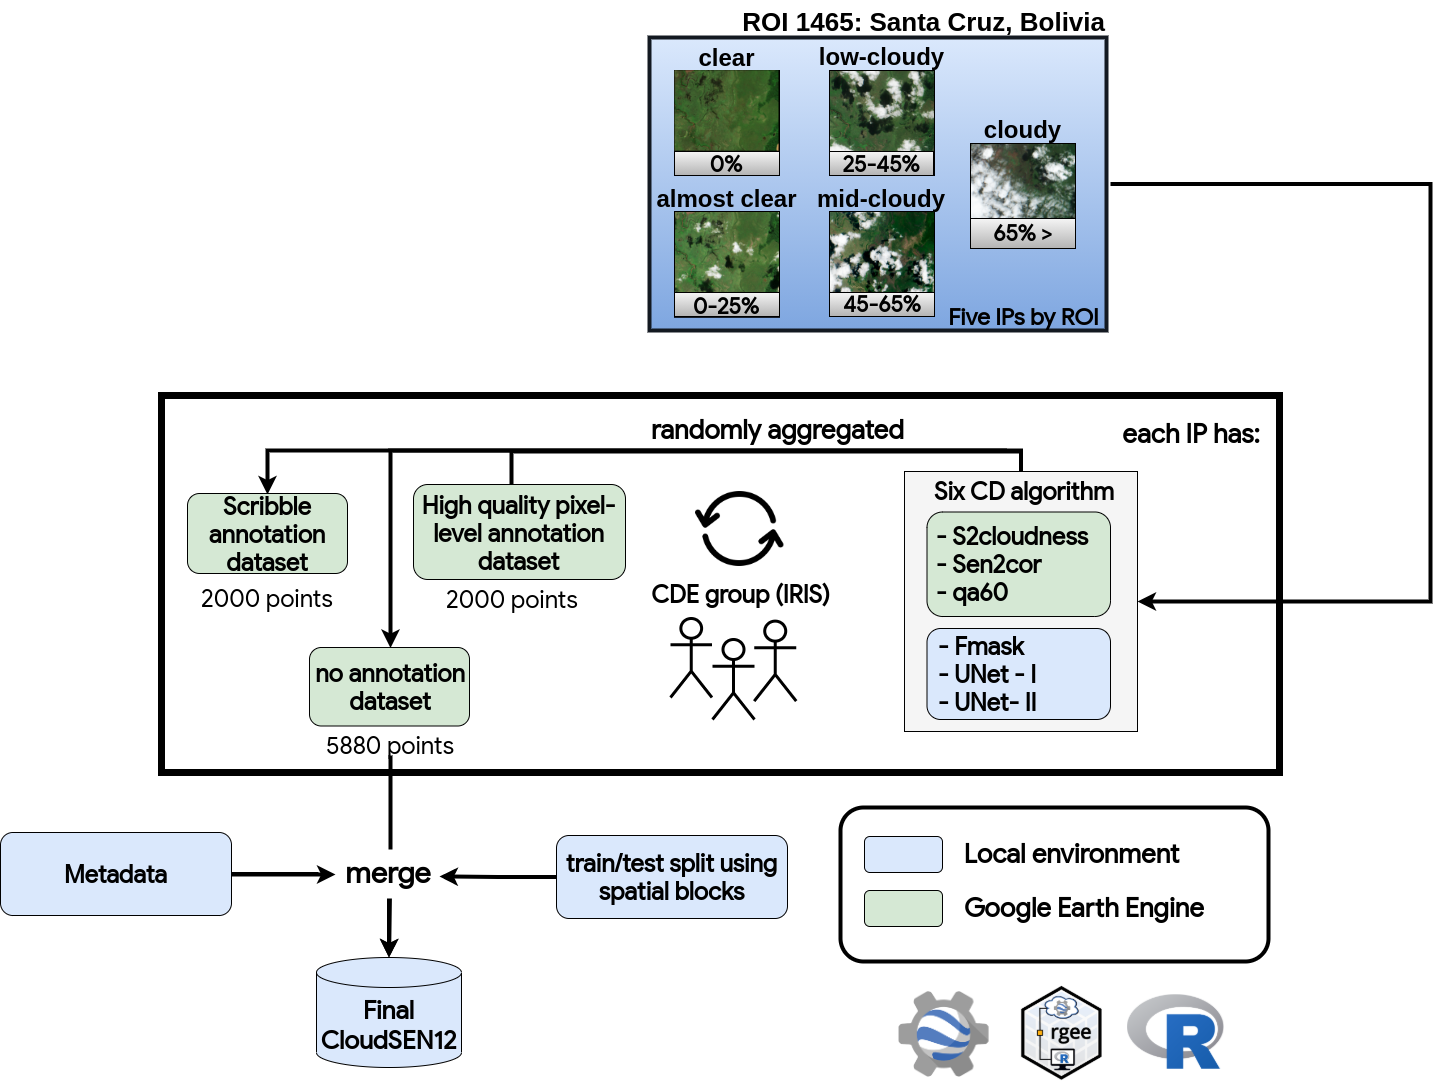
\includegraphics[width=1\textwidth]{images/methodology03.png}
				\label{fig:introfig02}
			\end{figure}
		\end{column}
		\begin{column}{0.3\textwidth}
			\begin{itemize}
				\item Add to each IP the results of 6 different CD algorithms. In addition, each ROI counts with manual labeling that can be of type: high-quality, scribble, or no annotation.
			\end{itemize}
		\end{column}
	\end{columns}
\end{frame}


\begin{frame}{CloudSEN12 - Labels}
\begin{figure}
	\centering
	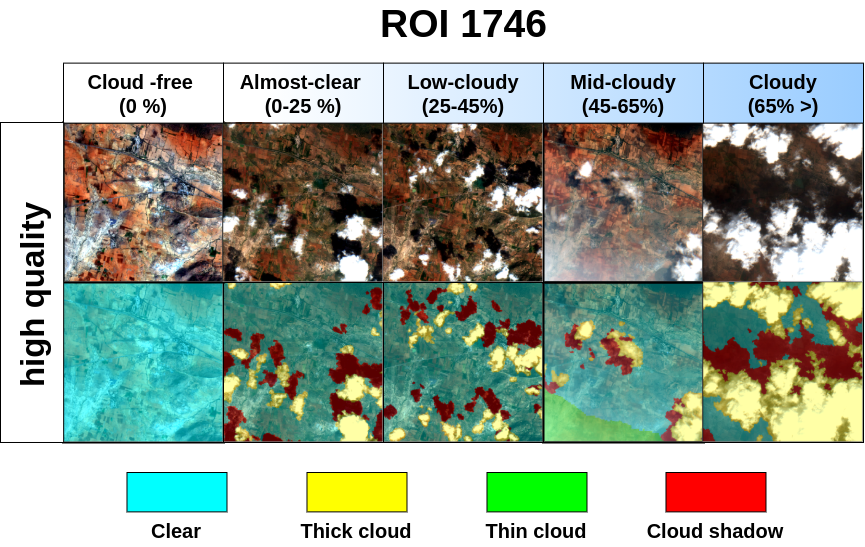
\includegraphics[width=0.7\linewidth]{images/labels01}
	\caption{}
	\label{fig:labels01}
\end{figure}
\end{frame}


\begin{frame}{CloudSEN12 - Labels}
	\begin{figure}
		\centering
		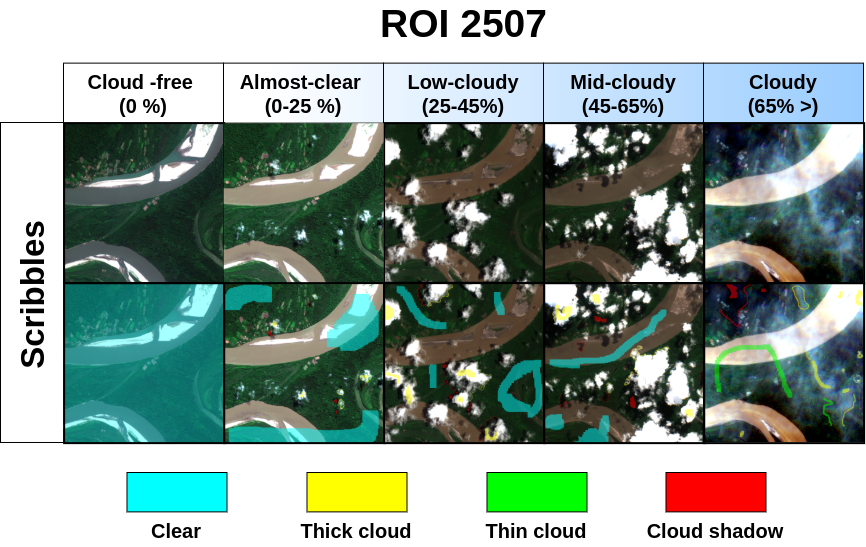
\includegraphics[width=0.7\linewidth]{images/labels02}
		\label{fig:labels01}
	\end{figure}
\end{frame}


\begin{frame}{CloudSEN12 - Labels}
	\begin{figure}
		\centering
		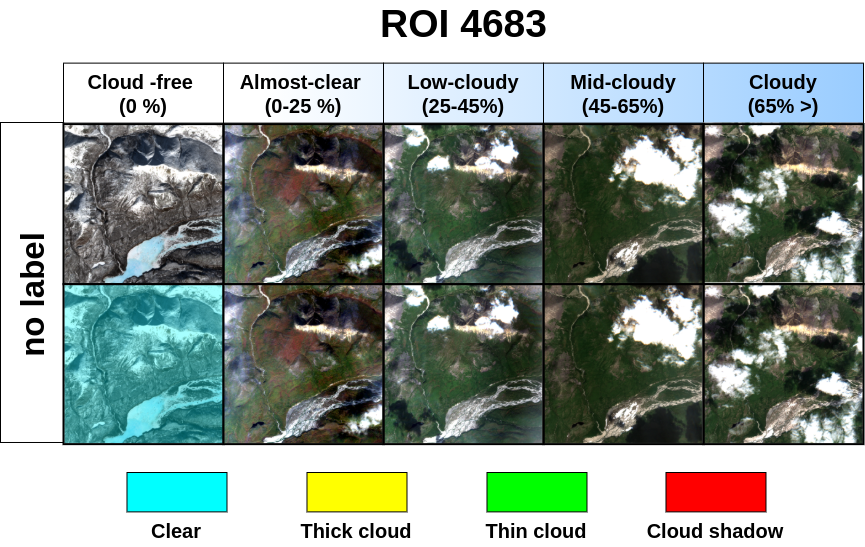
\includegraphics[width=0.7\linewidth]{images/labels03}
		\label{fig:labels01}
	\end{figure}
\end{frame}

\section{Methods}
\begin{frame}\frametitle{Overview}
\begin{itemize}
\pause \item The trivial Set Cover algorithm has running time of ${\cal O}(2^n)$.
\pause \item bla, bla, bla\ldots
\end{itemize}

\end{frame}

\section{Results}
\begin{frame}\frametitle{Overview}
\begin{itemize}
\pause \item The trivial Set Cover algorithm has running time of ${\cal O}(2^n)$.
\pause \item bla, bla, bla\ldots
\end{itemize}

\end{frame}

\section{Conclusions}
\begin{frame}\frametitle{Overview}
\begin{itemize}
\pause \item The trivial Set Cover algorithm has running time of ${\cal O}(2^n)$.
\pause \item bla, bla, bla\ldots
\end{itemize}

\end{frame}

%========================
% bibliography
%========================
%%%%%%%%%%%%%%%%%%
%
% bibliography
%
%%%%%%%%%%%%%%%%%%

\begin{frame} \frametitle{References}
\begin{thebibliography}{xx}\footnotesize

\bibitem{FominFVGrandoniFKratschD2009} {\sc Fomin FV, Grandoni F \& Kratsch D}, 2009, {\em A note on the complexity of minimum dominating set }, Journal of Discrete Algorithms, {\bf{4(2)}}, pp.\ 209--214.

\bibitem{critical} {\sc Grobler PJP \& Mynhardt CM}, 2009, {\em Secure domination critical graphs}, Discrete Mathematics, {\bf 309}, pp.~5820--5827.

\bibitem{VRB}{{\sc Van Rooij JMM \& Bodlaender HL}, 2011, {\em Exact algorithms for dominating set}, Discrete Applied Mathematics, {\bf 159}, pp.\ 2147--2164.}

\end{thebibliography}
\end{frame}

%=================================================
% end presentation
%=================================================
\begin{frame}
	\begin{center}
		\begin{figure}
			\centering
			
\includegraphics[width=0.8\linewidth]{images/goodbye.jpg}
			\label{fig:introfig01}
		\end{figure}
		\vspace{20px}
		\LARGE{Muchas gracias}	
	\end{center}
\end{frame}

% ----------------------------------------
% Extra slides ---------------------------
% ----------------------------------------

\begin{frame}{Context - II}
	\begin{columns}
		\begin{column}{0.5\textwidth}
			\begin{figure}
				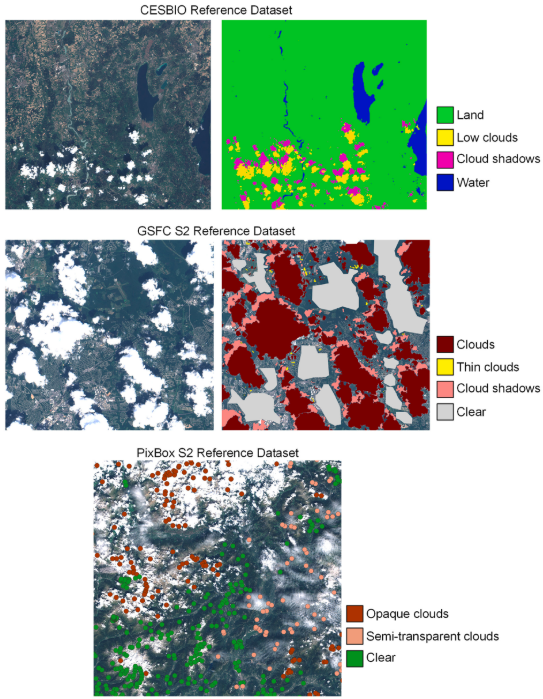
\includegraphics[width=0.85\textwidth]{images/contex_I.png}
				\caption[fig:introfig01]{Skakun et al. 2022}				
				\label{fig:introfig02}
			\end{figure}	
		\end{column}
		\begin{column}{0.5\textwidth}
			\begin{itemize}
				\item Cloud labels created by human photo-interpretation and ground-based camaras.
			\end{itemize}
		\end{column}
	\end{columns}
\end{frame}


\begin{frame}{Context - II}
	\begin{columns}
		\begin{column}{0.5\textwidth}
			\begin{figure}
				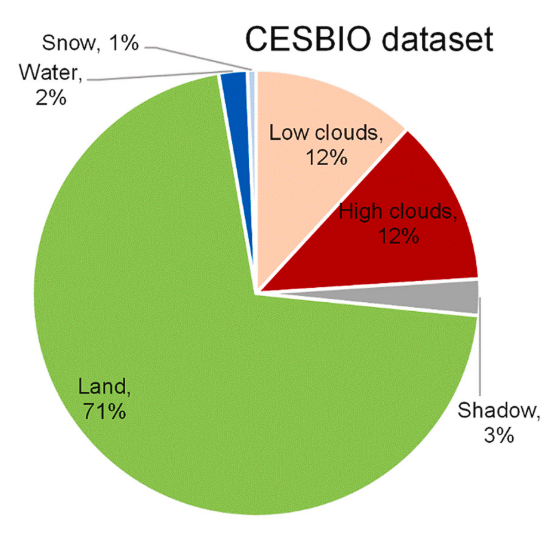
\includegraphics[width=0.85\textwidth]{images/contex_II.png}
				\caption[fig:introfig01]{Skakun et al. 2022}				
				\label{fig:introfig02}
			\end{figure}	
		\end{column}
		\begin{column}{0.5\textwidth}
			\begin{itemize}
				\item Cloud labels created by human photo-interpretation and ground-based camaras.
				\item High class imbalance.
			\end{itemize}
		\end{column}
	\end{columns}
\end{frame}

\begin{frame}{Context - II}
	\begin{columns}
		\begin{column}{0.5\textwidth}
			\begin{figure}
				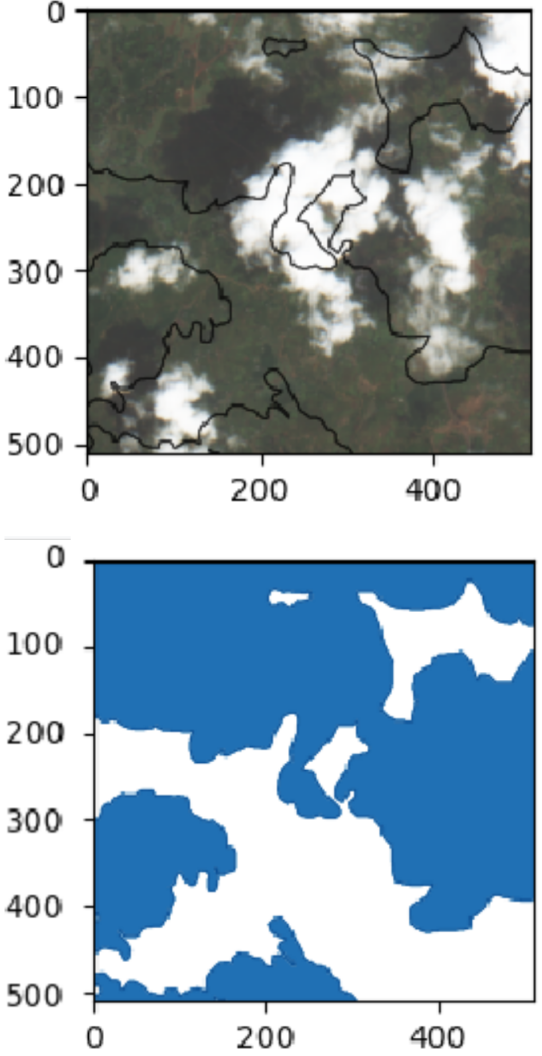
\includegraphics[width=0.6\textwidth]{images/contex_III.png}
				\label{fig:introfig02}
			\end{figure}	
		\end{column}
		\begin{column}{0.5\textwidth}
			\begin{itemize}
				\item Cloud labels created by human photo-interpretation, active learning and ground-based camaras.
				\item High class imbalance.
				\item \textbf{The quality of some datasets is poor.}
			\end{itemize}
		\end{column}
	\end{columns}
\end{frame}




\begin{frame}{Context - II}
	\begin{columns}
		\begin{column}{0.5\textwidth}
			\begin{figure}
				\includegraphics[width=0.95\textwidth]{images/intro_fig02_2.png}
				\label{fig:introfig02}
			\end{figure}	
		\end{column}
		\begin{column}{0.5\textwidth}
			\begin{itemize}
				\item Cloud labels created by human photo-interpretation and ground-based camaras.
				\item High class imbalance.	
				\item \textbf{The quality of some datasets is poor.}
				\item Created by \textbf{\textit{closed science practices}}.
				\item \textbf{No temporal features}.
			\end{itemize}
		\end{column}
	\end{columns}
\end{frame}




%% --------------------------------------------------------------

\begin{frame}{Quality Control}
	\begin{center}
		\begin{figure}
			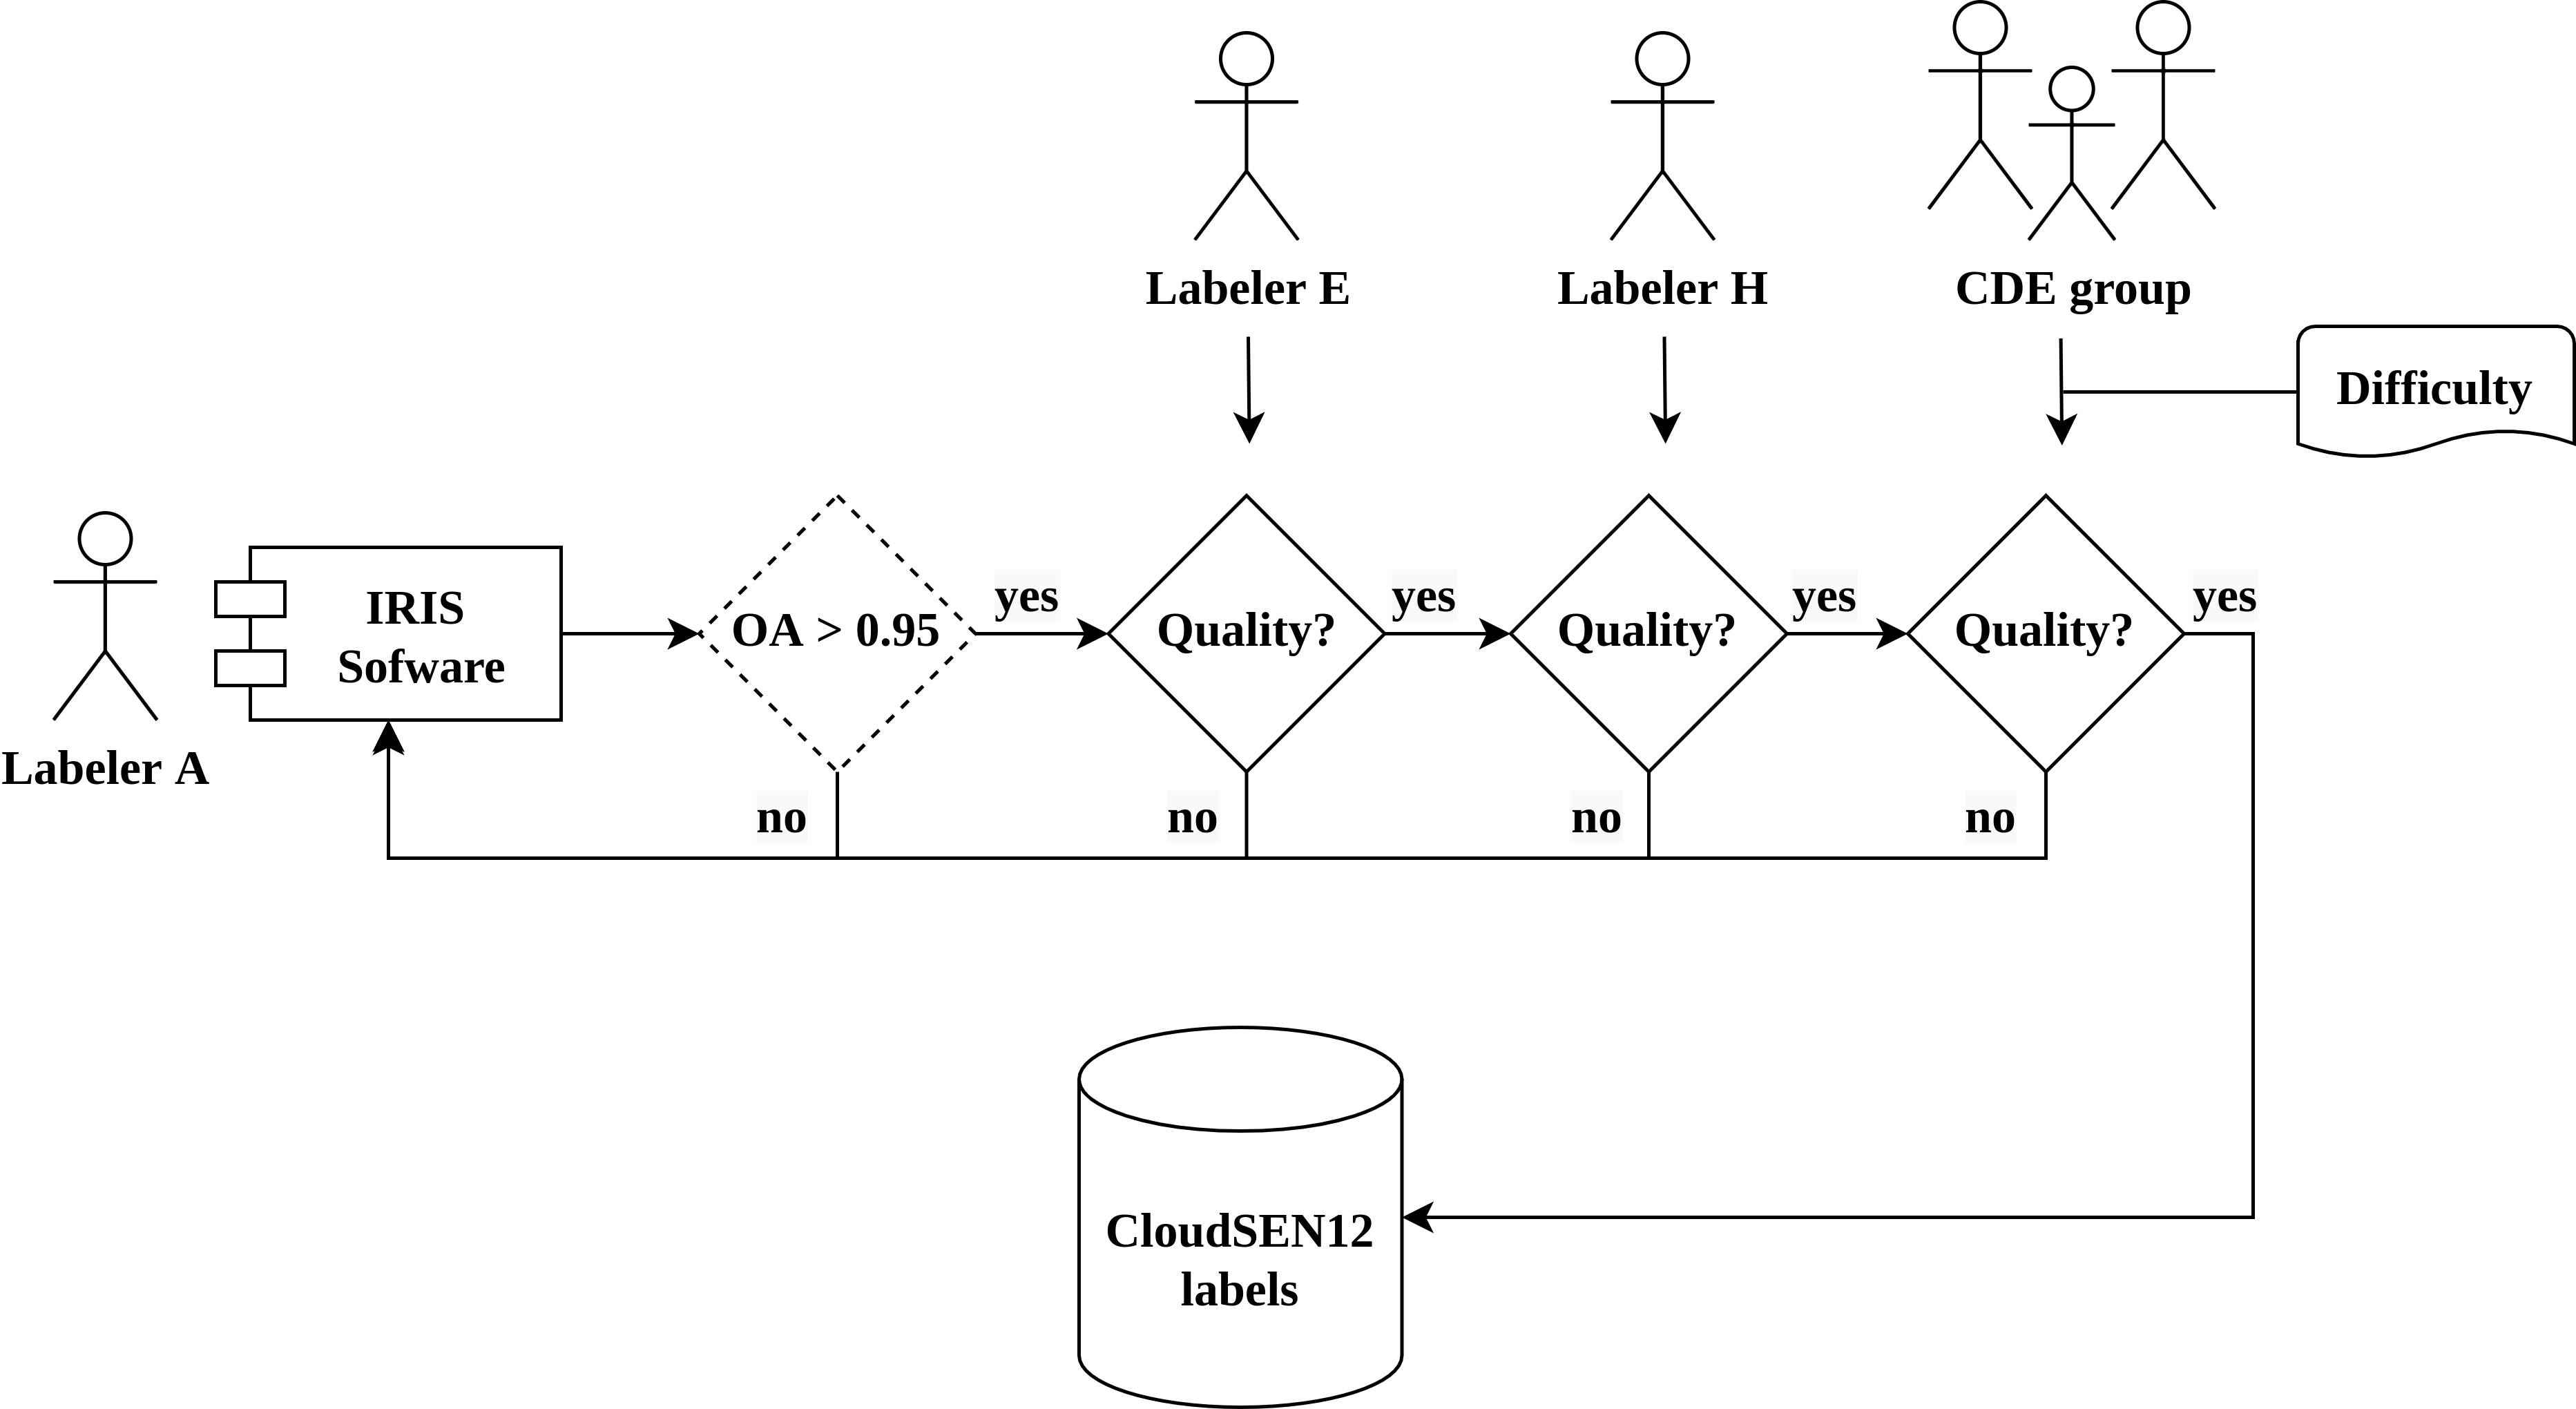
\includegraphics[width=0.9\linewidth]{images/figure08.png}
		\end{figure}
	\end{center}
\end{frame}



\begin{frame}{Dataset Structure}
	\begin{center}
		\begin{figure}
			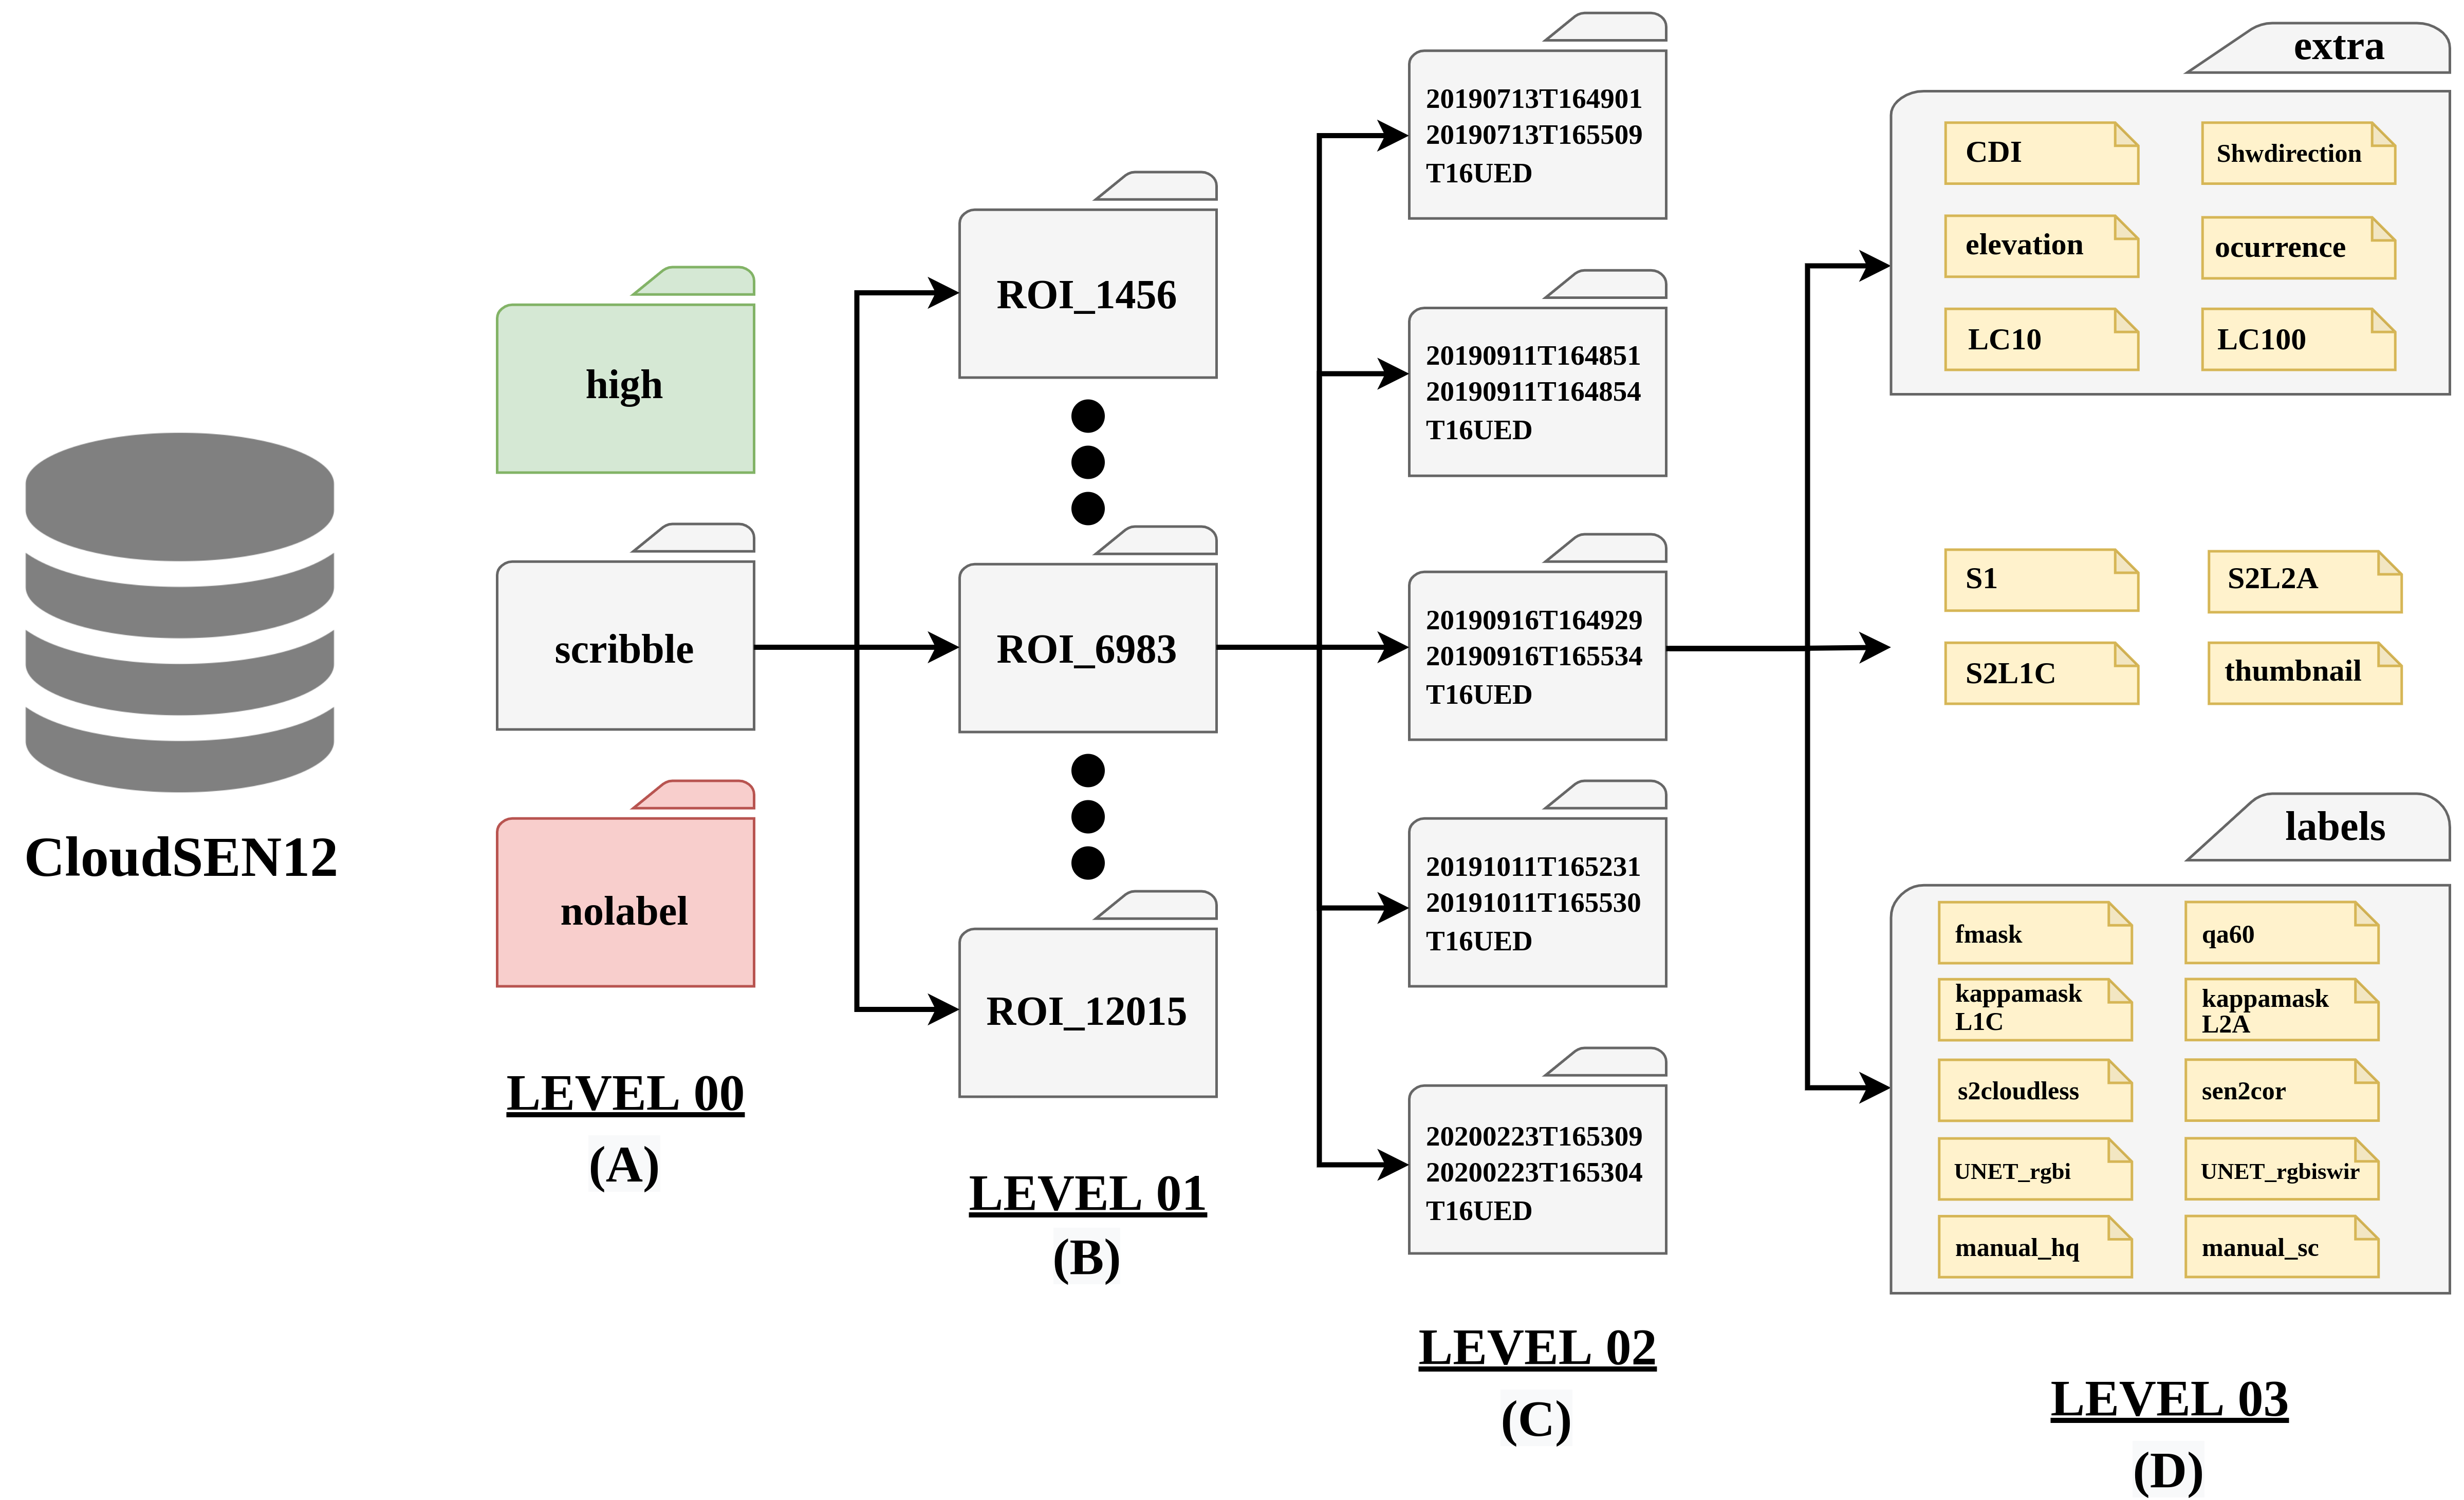
\includegraphics[width=0.8\linewidth]{images/figure10.png}
		\end{figure}
	\end{center}
\end{frame}



\begin{frame}{Technical validation}
	\begin{center}
		\begin{figure}
			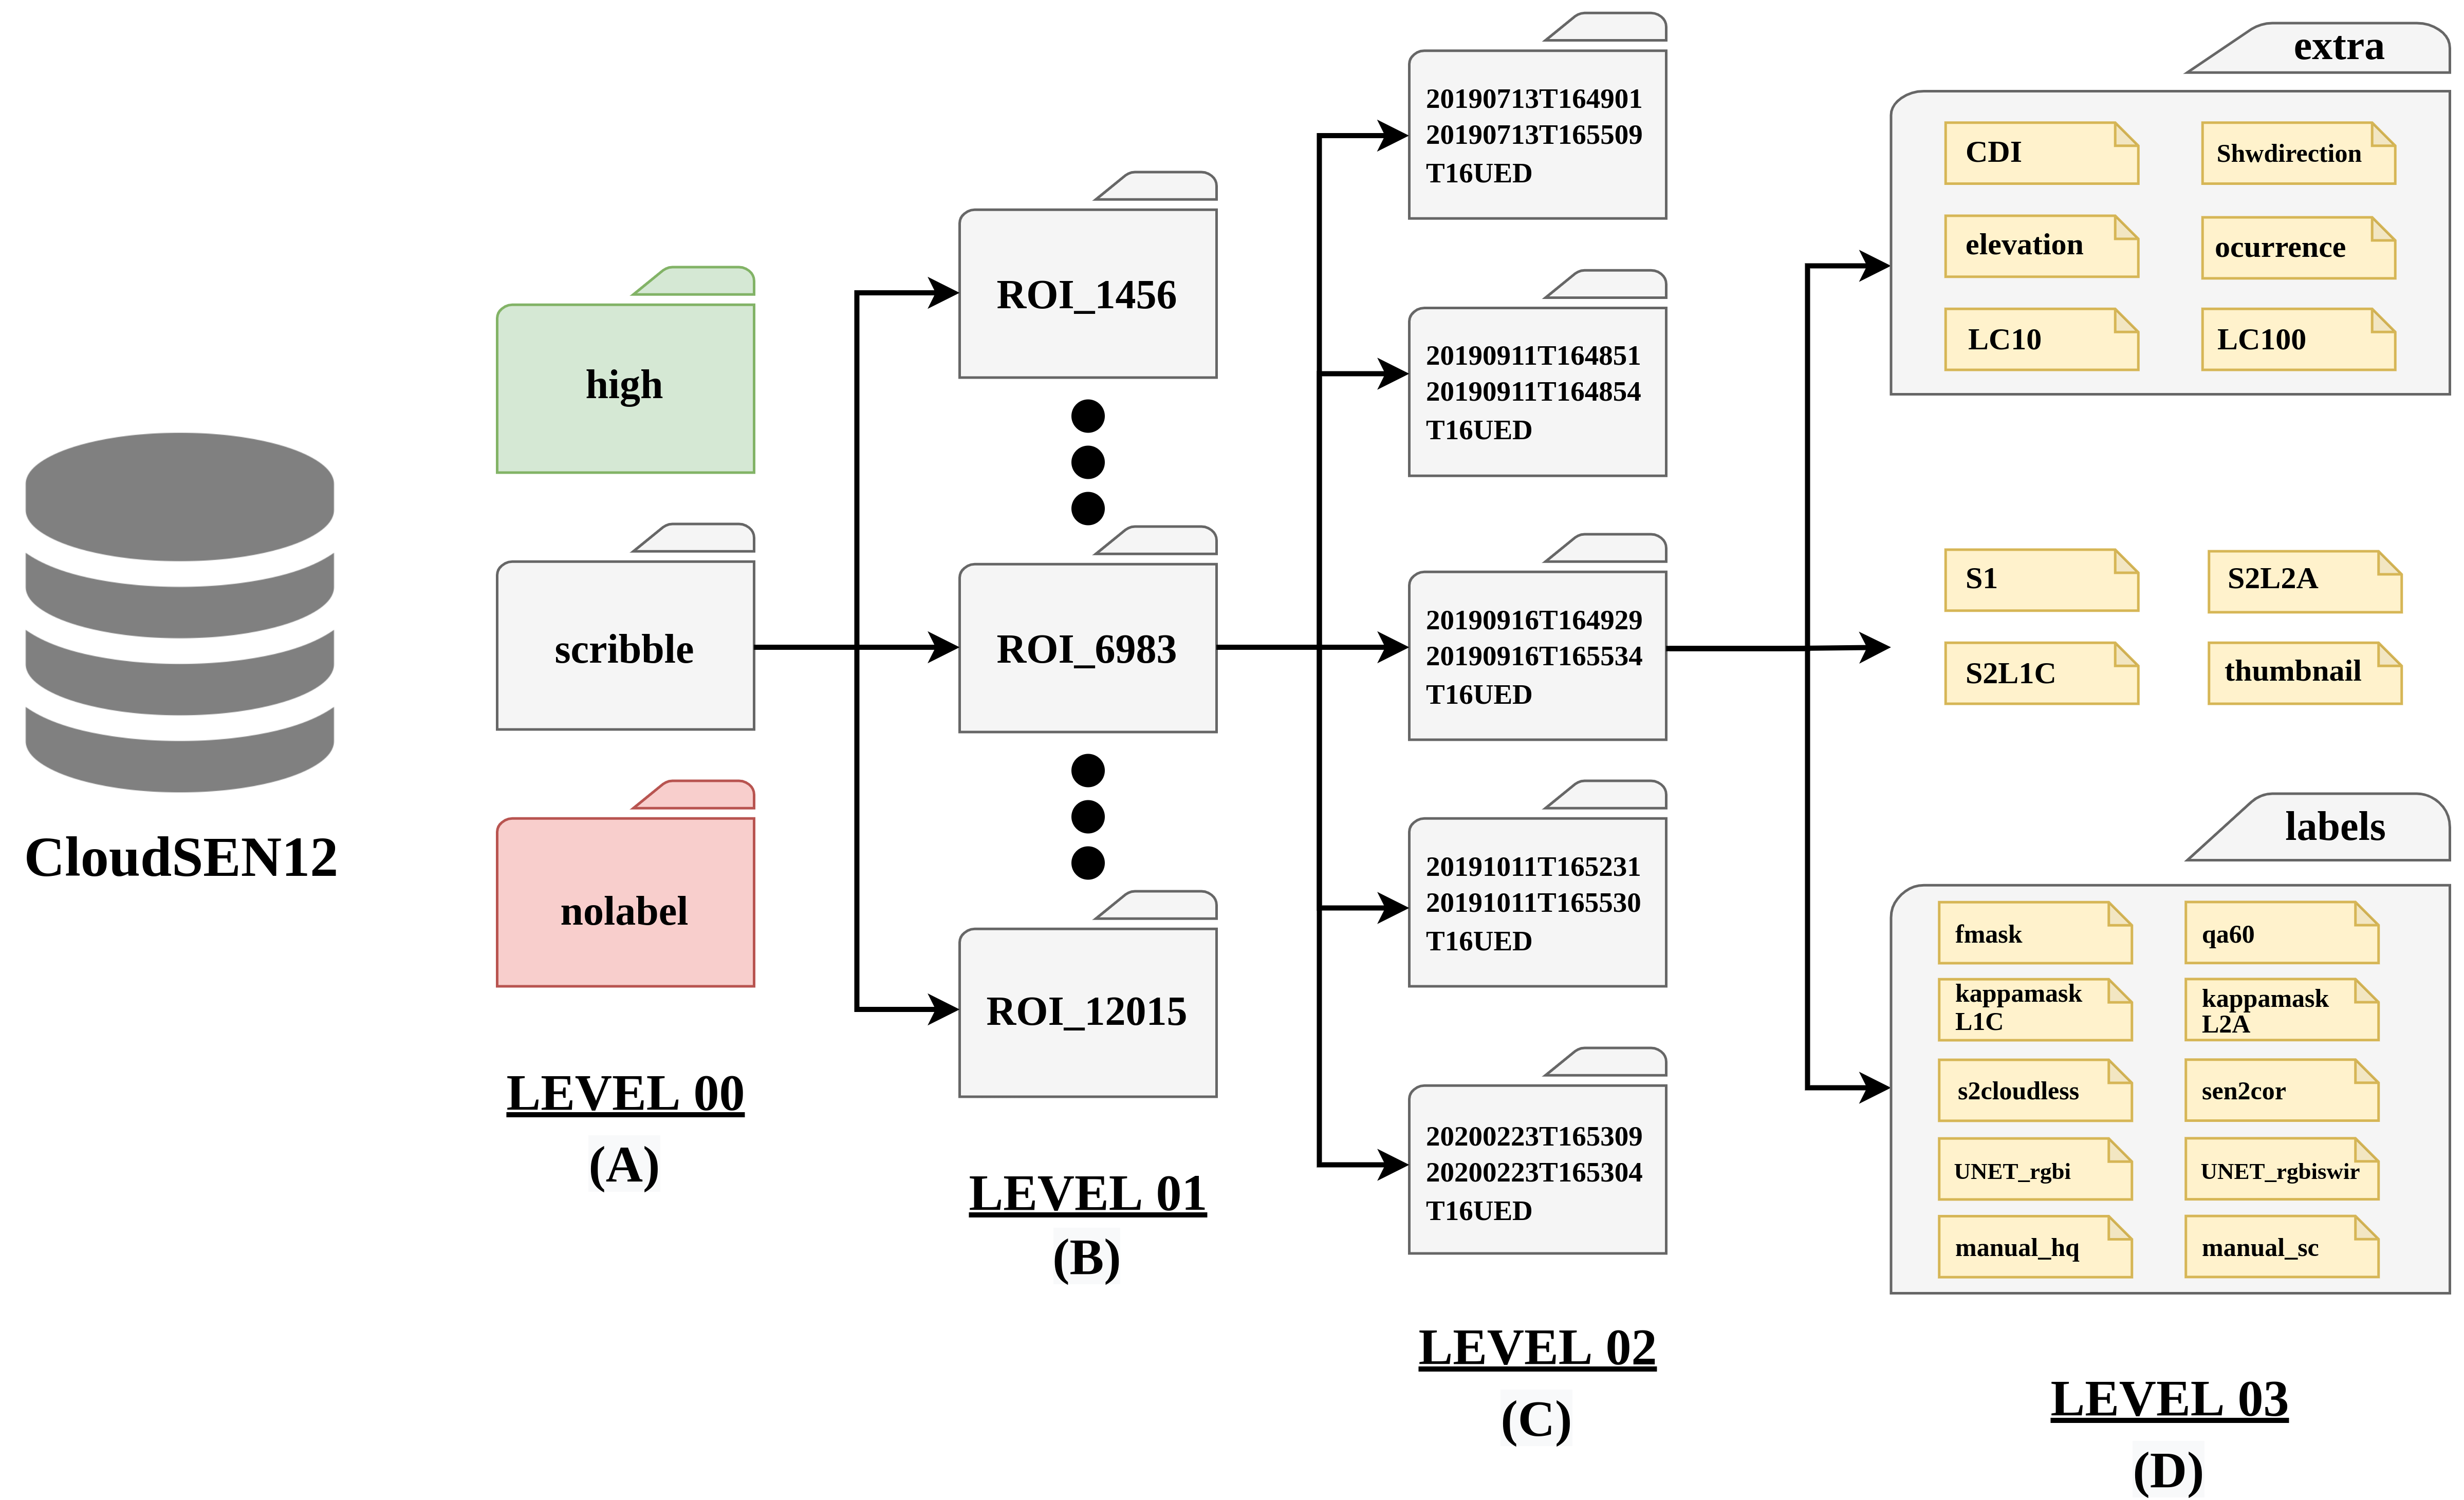
\includegraphics[width=0.6\linewidth]{images/figure10.png}
		\end{figure}
	\end{center}
\end{frame}


\end{document}